
\documentclass[11pt,a4paper]{article}

% Essential packages
\usepackage[utf8]{inputenc}
\usepackage[T1]{fontenc}
\usepackage[margin=1in]{geometry}
\usepackage{amsmath,amsfonts,amssymb}
\usepackage{graphicx}
\usepackage{booktabs}
\usepackage{url}
\usepackage{hyperref}
\usepackage{natbib}
\usepackage{setspace}


% Additional useful packages
\usepackage{fancyhdr}
\usepackage{subcaption}
\usepackage{tikz}
\usepackage{algorithm}
\usepackage{algorithmic}
\usepackage{listings}
\usepackage{xcolor}

% Configure hyperref
\hypersetup{
    colorlinks=true,
    linkcolor=blue,
    filecolor=magenta,      
    urlcolor=cyan,
    citecolor=blue,
    pdftitle={Your Paper Title},
    pdfauthor={Your Name},
}

% Set line spacing
\doublespacing

% Configure headers and footers
\pagestyle{fancy}
\fancyhf{}
\rhead{\thepage}
\lhead{\textit{Data Project Report}}
\renewcommand{\headrulewidth}{0.4pt}

% Title page information
\title{Data Project Report}

\author{
    Tate Mason\thanks{Tate.Mason@uga.edu} \\
    \textit{John Munro Godfrey Sr. Department of Economics} \\
    \textit{The University of Georgia} \\
    \textit{Athens, Georgia} \\
    \\
}

\date{\today}

% Abstract environment
\newenvironment{abstract}%
{\cleardoublepage\null \vfill\begin{center}%
\bfseries \abstractname \end{center}}%
{\vfill\null}

\begin{document}

% Title page
\maketitle
\thispagestyle{empty}

\subsection{Datasets}
\label{subsec:datasets}

My primary datasource is the IPUMS USA dataset, which provides detailed microdata on individuals' demographic, economic, and housing characteristics in the United States. I will focus on individuals between the ages of 40 and 80, analyzing their migration patterns throughout their lifetime. To supplement the decennial census data from IPUMS, I will also use the American Community Survey (ACS), which offers annual data for a smaller subset of the population. I can link this annual data to the decennial census via a serial number, allowing me to track individuals' migration decisions over time, along with other relevant characteristics such as income and housing conditions.

More specifically, I will extract wages via computing the average wage income for individuals in each state. I also compute amenity indices for each state, where workers value transportation time to work, taken from IPUMS, and retirees value the climate, taken from NOAA data\footnote{Cooling degree days calculated as in Kennan and Walker (2011)}. Housing costs are computed by taking the average rent paid by renters in each state. Health care costs are computed using data from the CMS on average Medicare spending per enrollee in each state. 

The data spans from 2000-2019, covering the 2000 and 2010 decennial censuses, as well as all interyear data from the ACS. This gives me a comprehensive view of migration patterns over two decades. All dollar amounts are normalized to 2010 dollars using the CPI index from the BLS. I restrict my sample to heads of household to simplify computaion, and I drop individuals who reside in group quarters, such as nursing homes or prisons, as their migration decisions may be influenced by factors not captured in the model.

\subsection{Summary Statistics}
\label{subsec:summary_statistics}

When looking at the summary statistics for individuals aged 40-80 in the IPUMS and ACS datasets, I find a total sample size of 21,138,046 individuals. The average age in this group is 57.62 years. The mean wage income is \$33,251.83, while the average gross rent paid by renters is \$170.07 per month. Health care costs average \$6,336.11 annually for retirees in this age group. Approximately 17\% of individuals in this cohort moved to a different state within the observed period.

\begin{table}[htbp]
\centering
\caption{Summary Statistics}
\label{tab:summ_stats}
  \begin{tabular}{|l|c|}
    \hline
    \hline
    n & 21,138,046 \\
    Average Age & 57.62 \\
    Average Wages & 33251.83 \\
    Average Gross Rent & 170.07\\
    Average Health Costs & 6336.11 \\
    Mover \% & 17\% \\
    \hline
  \end{tabular}
\end{table}

Next, I examine migration patterns by age. I create age profiles, plotting the probability of moving against two year age bins. The results show that the probability of moving peaks around age 65 until age 69. This implies there are a lot of movers around retirement age, which may suggest that individuals are making relocation decisions based on retirement plans and non-career factors.

\begin{figure}[htbp]
  \centering
  \caption{Age Profile of Movers}
  \label{fig:age_profile}
  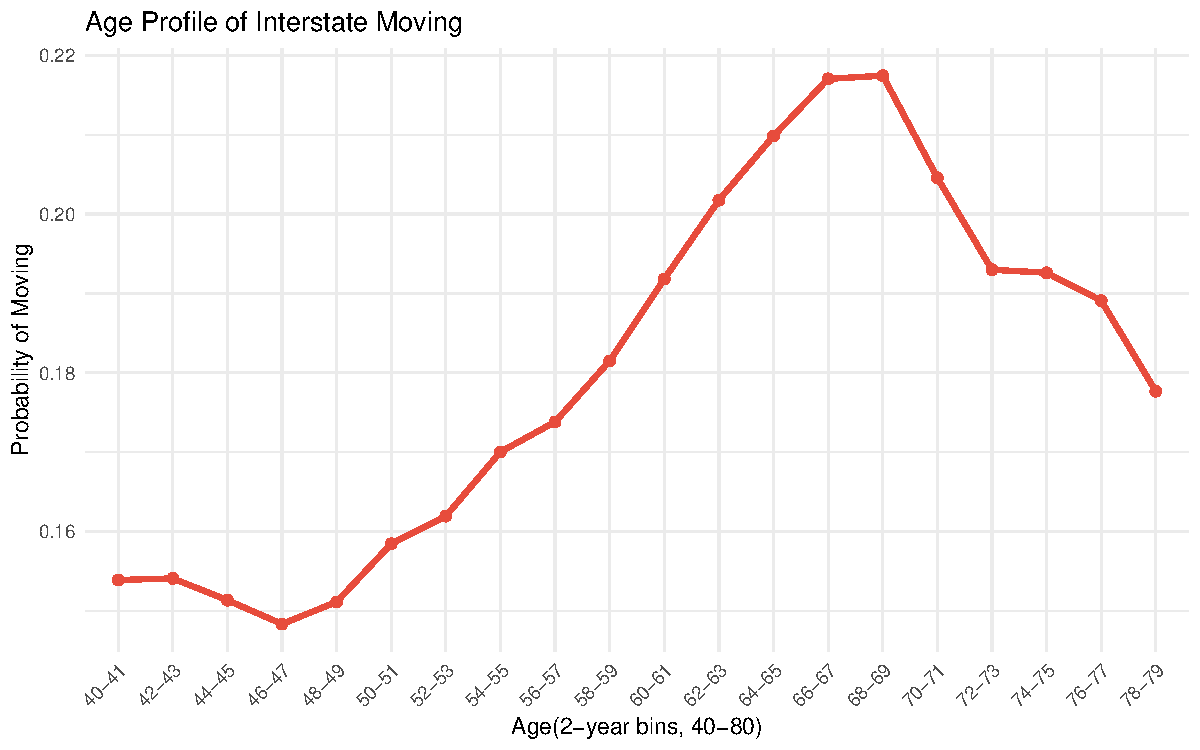
\includegraphics[width=0.7\textwidth]{final_pres/figures/age_profile_move.pdf}
\end{figure}

Further, I analyze migration patterns by different agent characteristics. I find that higher education levels are associated with higher mobility rates. The probability of moving increases as one climbs the educational attainment ladder, with those holding at least a bachelor's degree being the most mobile. Income shows similar patterns, where individuals in higher income brackets exhibit greater mobility. Additionally, the presence of children in the household reduces the likelihood of moving, suggesting that family considerations play a significant role in relocation decisions. Interestingly, marital status influences mobility such that married individuals are more likely to move compared to their single counterparts, possibly due to dual-income households having more flexibility in relocation or the fact that there are now two individuals to consider in the decision-making process.

\begin{figure}[htbp]
  \centering
  \begin{subfigure}{0.45\textwidth}
    \centering
    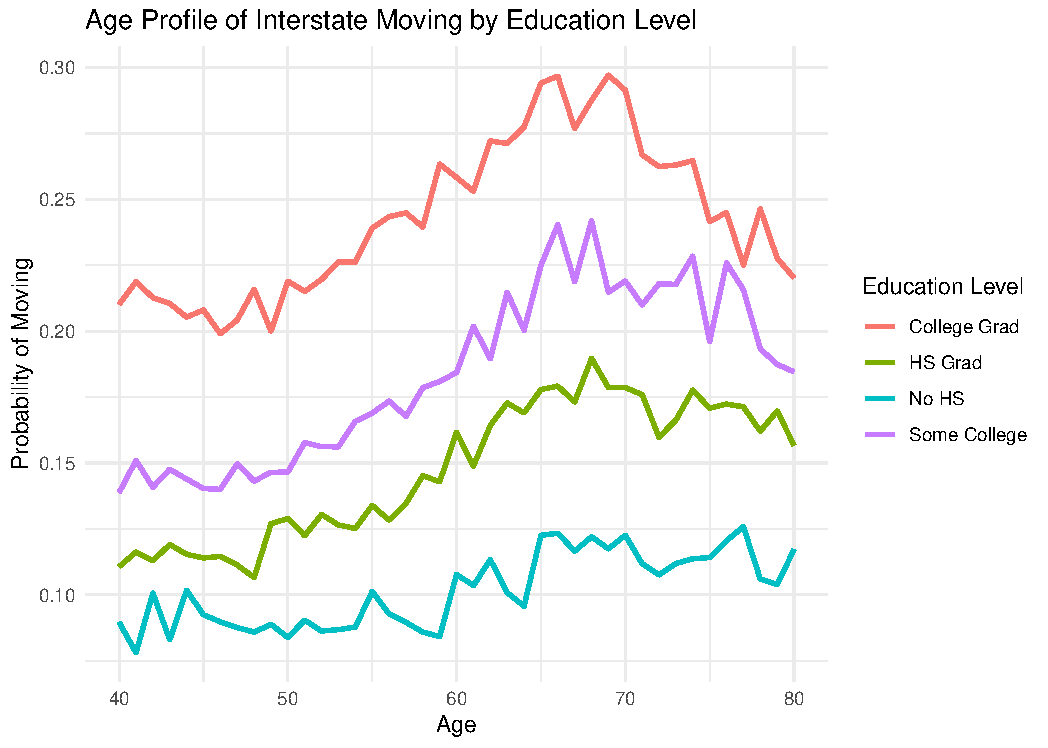
\includegraphics[width=\textwidth]{final_pres/figures/mover_prop_educ.pdf}
    \caption{Mobility by Education Level}
    \label{fig:edu_profile}
  \end{subfigure}
  \hfill
  \begin{subfigure}{0.45\textwidth}
    \centering
    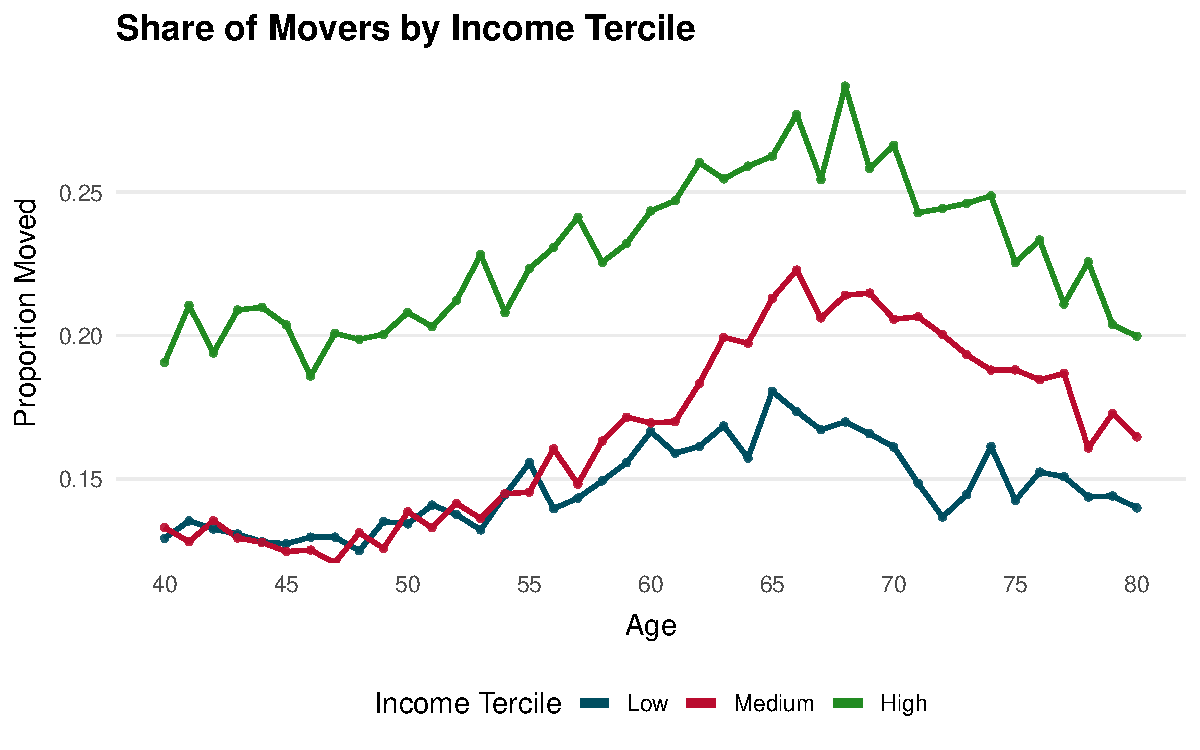
\includegraphics[width=\textwidth]{final_pres/figures/mover_prop_income.pdf}
    \caption{Mobility by Income Level}
    \label{fig:income_profile}
  \end{subfigure}
  \caption{Mobility Patterns by Agent Characteristics}
  \label{fig:mobility_patterns}
\end{figure}

\begin{figure}[htbp]
  \centering
  \begin{subfigure}{0.45\textwidth}
    \centering
    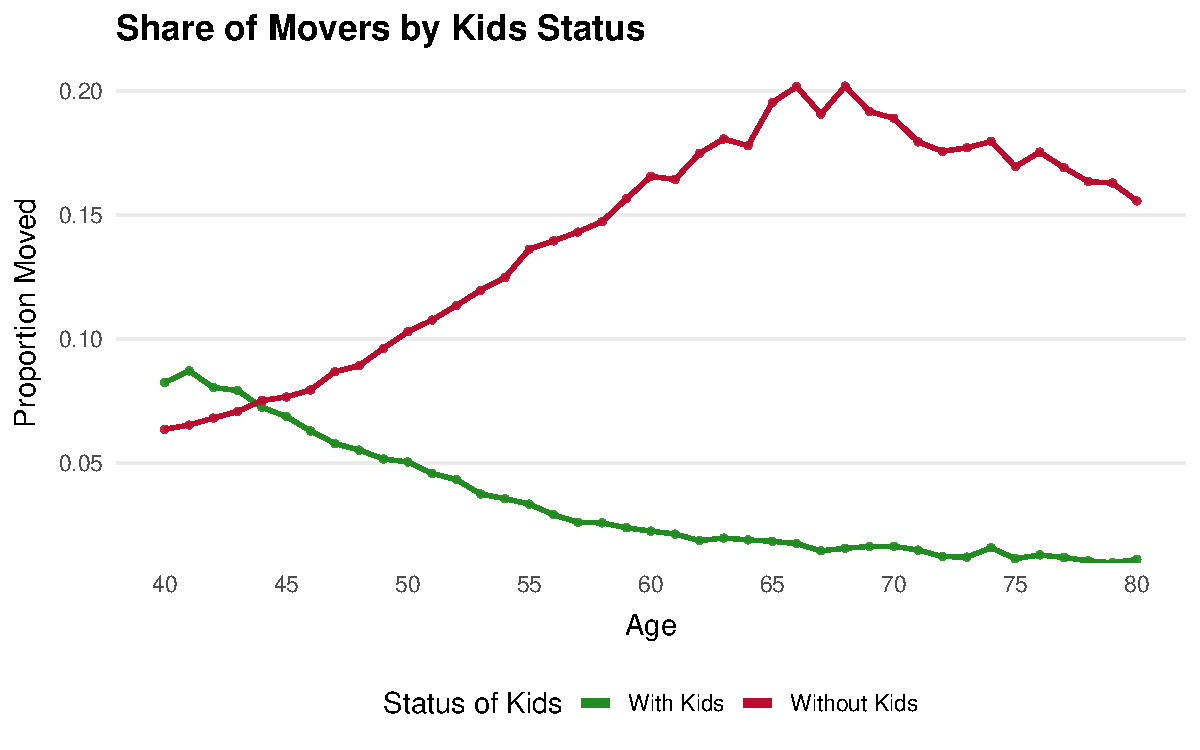
\includegraphics[width=\textwidth]{final_pres/figures/mover_prop_kids.pdf}
    \caption{Mobility by Presence of Children}
    \label{fig:kid_profile}
  \end{subfigure}
  \hfill
  \begin{subfigure}{0.45\textwidth}
    \centering
    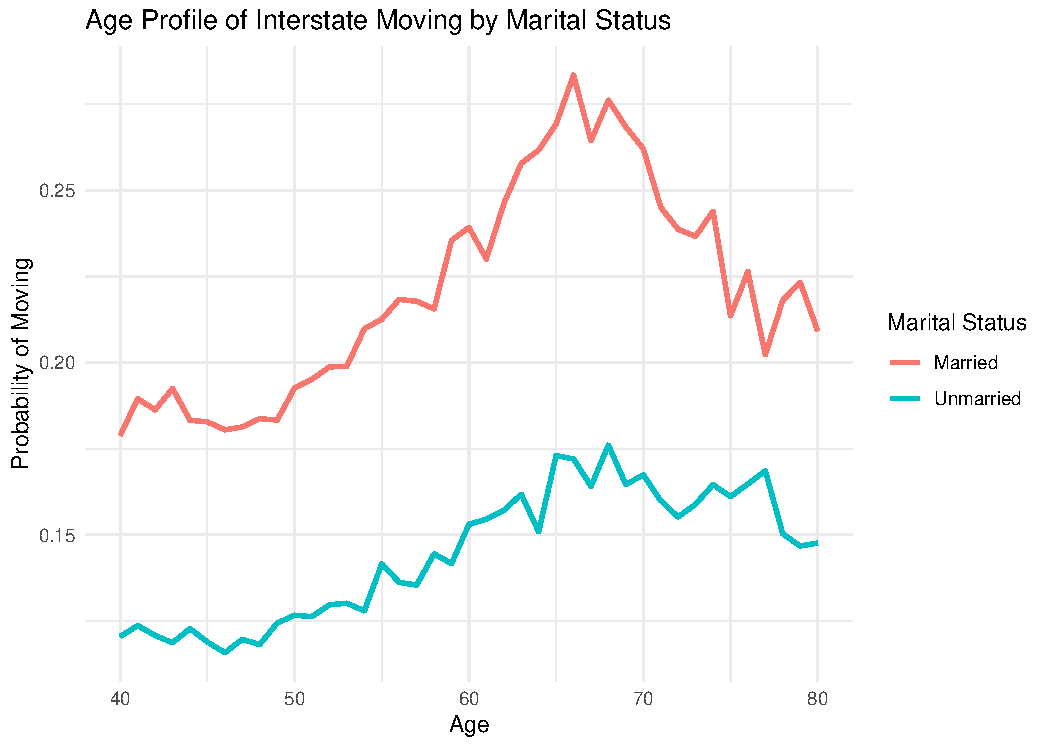
\includegraphics[width=\textwidth]{final_pres/figures/mover_prop_marst.pdf}
    \caption{Mobility by Marital Status}
    \label{fig:marst_profile}
  \end{subfigure}
  \caption{Mobility Patterns by Family Characteristics}
  \label{fig:family_mobility_patterns}
\end{figure}

Finally, having a baseline understanding of migration flows in the data is crucial for calibrating the structural model and validating its predictions against observed patterns. Below, I present heat maps showing migration flows between states for workers and retirees. The intensity of the color indicates the volume of movers between each pair of states. These visualizations help identify popular destinations and origins for both groups, providing insights into how career and non-career factors influence relocation decisions.

\begin{figure}[htbp]
  \centering
  \begin{subfigure}{0.45\textwidth}
    \centering
    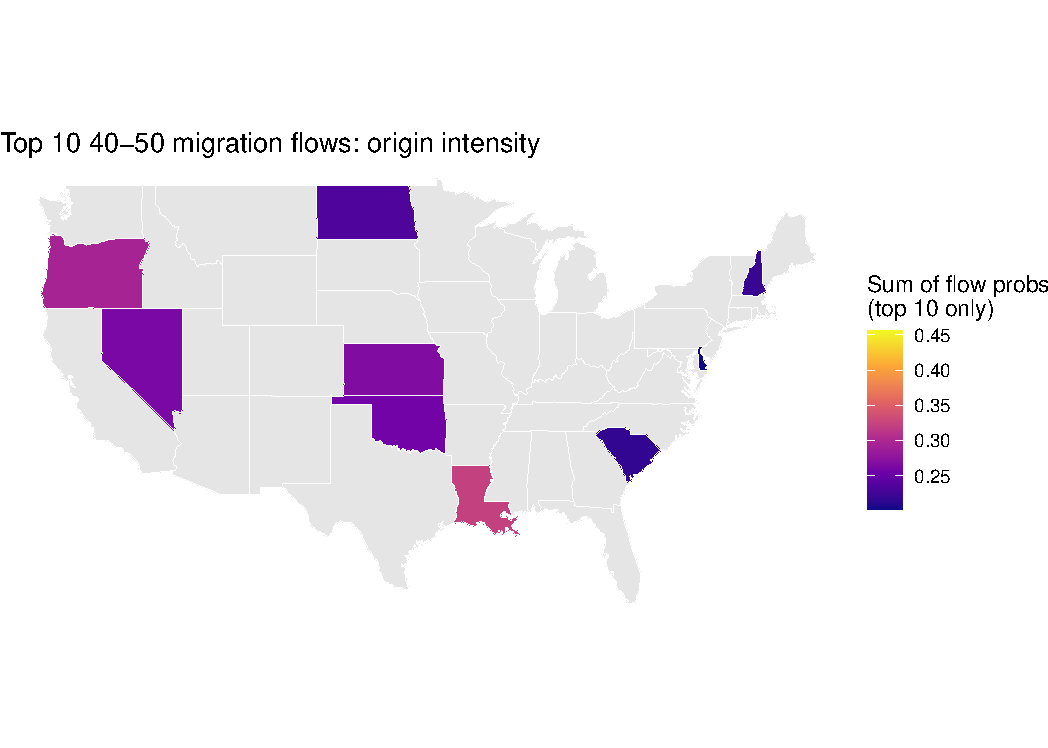
\includegraphics[width=\textwidth]{final_pres/figures/map_40_50_origins.pdf}
    \caption{Worker Migration Origins}
    \label{fig:worker_origin_heatmap}
  \end{subfigure}
  \hfill
  \begin{subfigure}{0.45\textwidth}
    \centering
    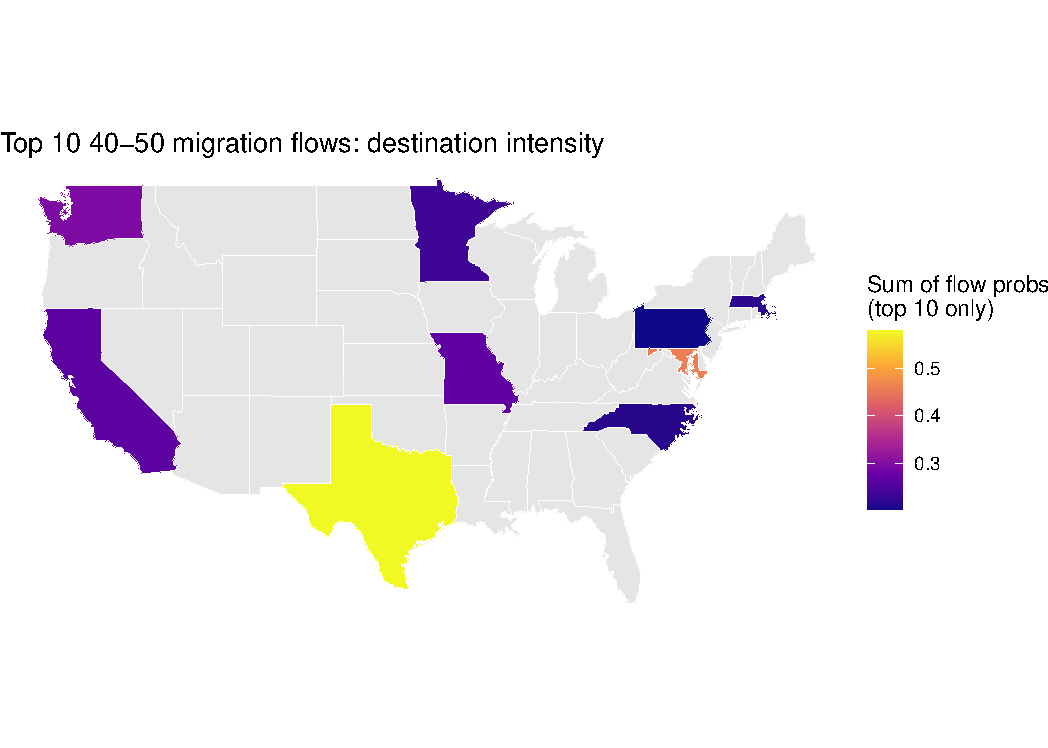
\includegraphics[width=\textwidth]{final_pres/figures/map_40_50_dests.pdf}
    \caption{Worker Migration Destinations}
    \label{fig:worker_dest_heatmap}
  \end{subfigure}
  \caption{Worker Migration Heatmaps}
  \label{fig:worker_heatmaps}
\end{figure}

The figures show that workers tend to move to states in proximity of their current states which also have strong job markets, such as California, Texas, and Florida.

\begin{figure}[htbp]
  \centering
  \begin{subfigure}{0.45\textwidth}
    \centering
    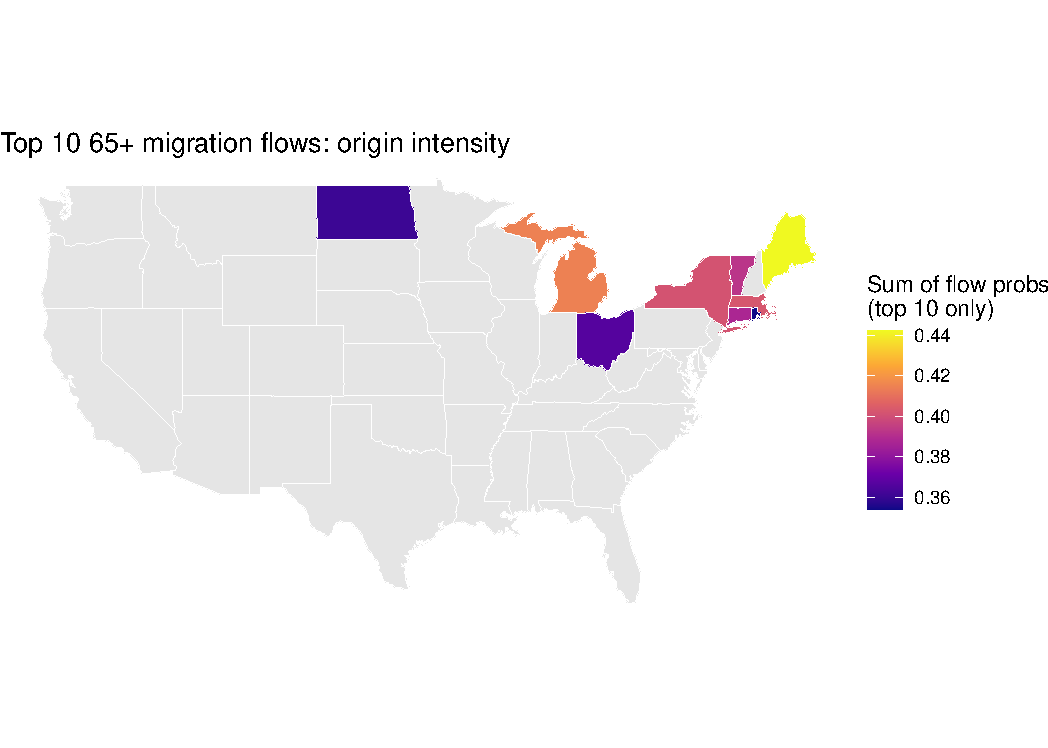
\includegraphics[width=\textwidth]{final_pres/figures/map_65p_origins.pdf}
    \caption{Retiree Migration Origins}
    \label{fig:retiree_origin_heatmap}
  \end{subfigure}
  \hfill
  \begin{subfigure}{0.45\textwidth}
    \centering
    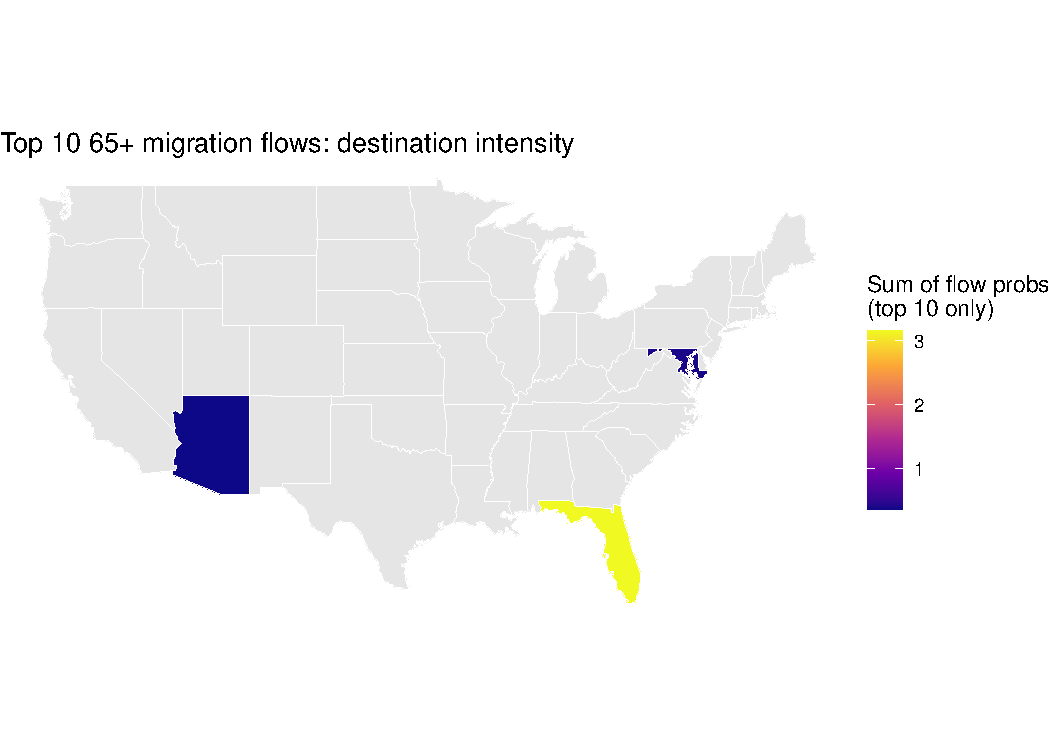
\includegraphics[width=\textwidth]{final_pres/figures/map_65p_dests.pdf}
    \caption{Retiree Migration Destinations}
    \label{fig:retiree_dest_heatmap}
  \end{subfigure}
  \caption{Retiree Migration Heatmaps}
  \label{fig:retiree_heatmaps}
\end{figure}

Retirees, on the other hand, show a strong preference for moving to states with favorable climates and lower costs of living, such as Florida and Arizona. These patterns highlight the differing motives for migration between workers and retirees, which the structural model aims to capture.
